\section{Cascaded Shadow Maps}

\begin{figure}[h]
    \centering
    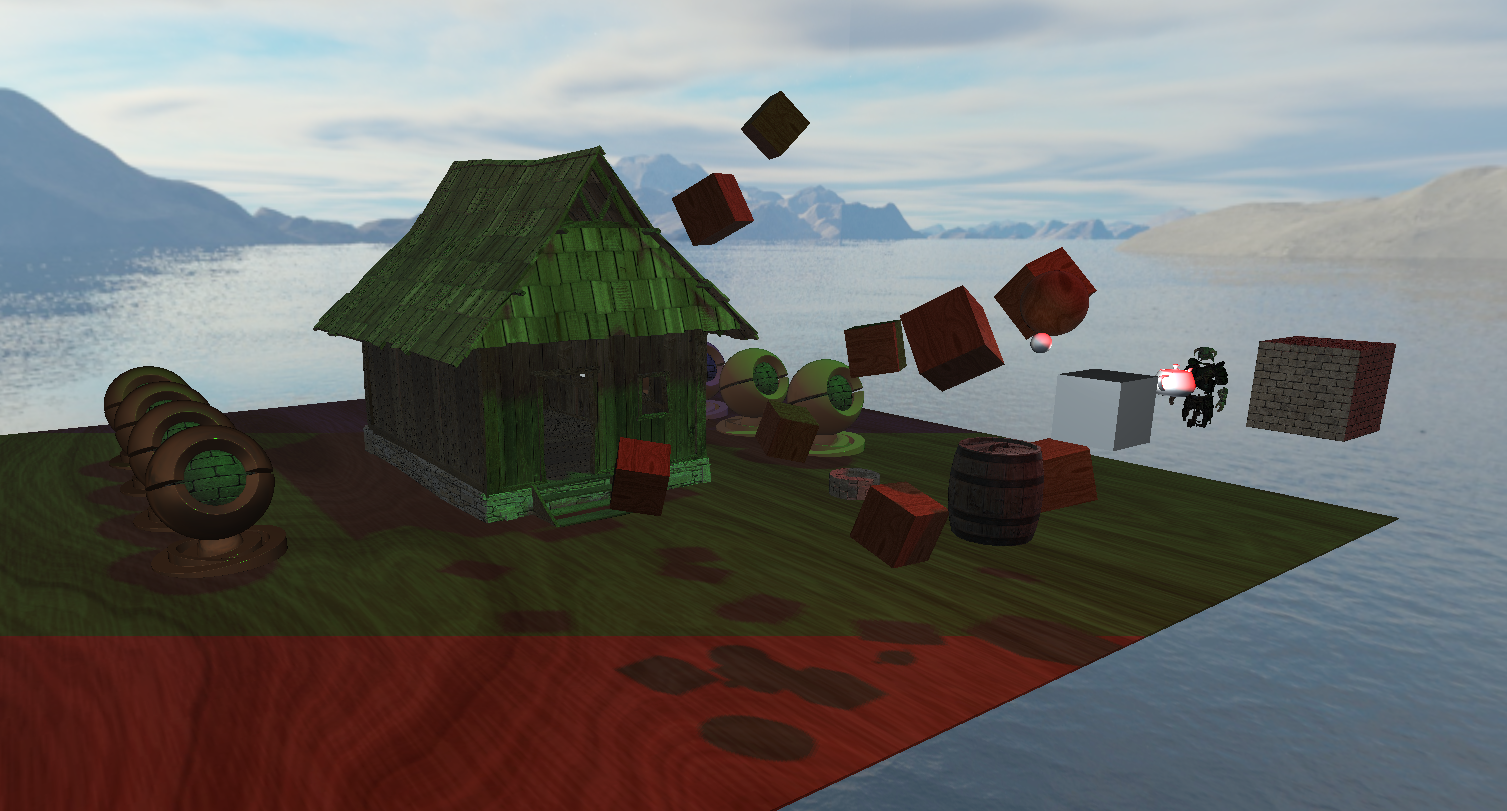
\includegraphics[scale=0.25, clip=true]{./image/csmsplits.png}
    \caption{Visualized frustum splits}
\label{fig:csmsplits}
\end{figure}

\begin{figure}[b]
    \centering
    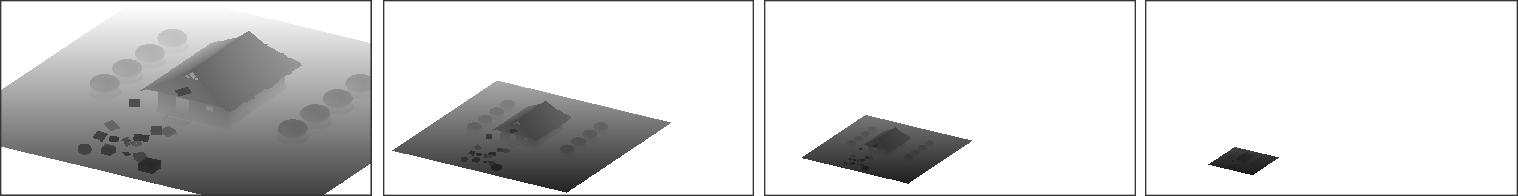
\includegraphics[scale=0.3, clip=true]{./image/csmbufs.png}
    \caption{Depth maps for each frustum split}
\label{fig:csmbufs}
\end{figure}

In order to implement shadows in the scenes the use of some Shadow Mapping technique was required.
The simple shadow mapping algorithm would not be sufficient for large space scenes. Using just
a single shadowmap leads to difficulties in adjusting the shadow map to avoid surface acne and aliasing
problems. Also this would require a very high and impractical resolution in order capture both large
space scenes and being able to show desirable detail. Cascaded Shadow Maps is an approach that helps bypass
these problems by providing higher resolution of the depth texture near the viewer an lower resolution far
away. This is achieved by splitting the camera view frustum and creating a separate depth-map for each
partition (see Figures~\ref{fig:csmsplits},\ref{fig:csmbufs}). The algorithm is composed of two main parts:

\begin{enumerate}
\item For every frustum split render the scene depth from the light pov
\item While rendering the scene from the camera pov, pick and use the matching shadow map for the current
    fragment's Z value
\end{enumerate}
